% Estamos acá:
% \subsection{Optimización de \texttt{min_df} y \texttt{max_df}}%
% \label{sub:minmaxdf}

Se realizaron mediciones sobre el \textit{accuracy} al variar los valores de
\texttt{min\_df} y \texttt{max\_df} para la mejor configuración de parámetros
conocida hasta el momento de realizar este experimento ($k=1800$, sin PCA).

\begin{figure}[h]
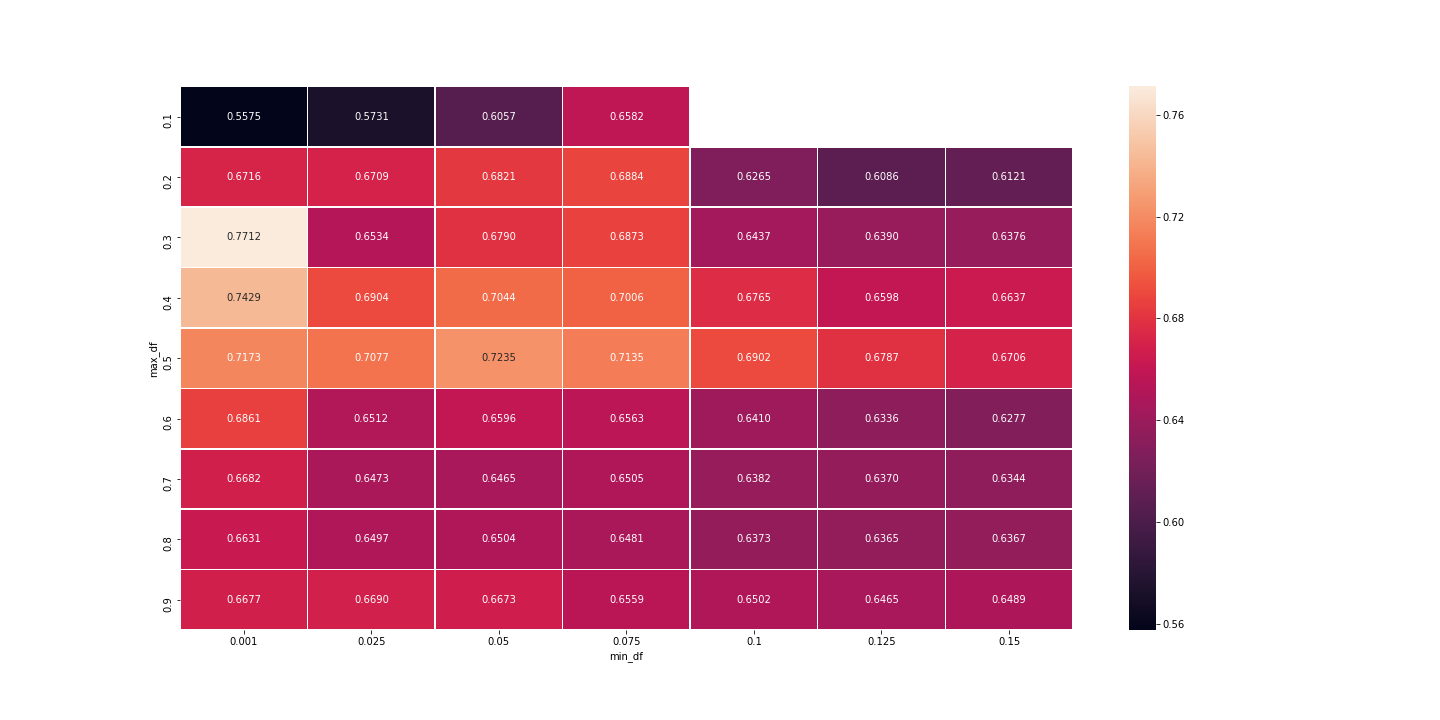
\includegraphics[width=\textwidth]{./img/exp_maxmindf.png}
\centering
\caption{
Valores de \textit{accuracy} para un \textit{grid search} sobre
\texttt{min\_df} y \texttt{max\_df} para el modelo de KNN sin PCA y $k=1800$.
Se obtuvo un mejor rendimiento al probar nuevas configuraciones del
vectorizador.
}
\label{fig:param-big}
\end{figure}

Como resultado, se obtuvo para $\mathtt{min\_df}=0.001$ y
$\mathtt{max\_df}=0.3$ un \textit{accuracy} de $0.77$, el mejor valor alcanzado
hasta el momento.

Puede verse que con un ligero aumento de \texttt{min\_df}, el modelo pierde
eficacia. Por otro lado, los mejores resultados fueron obtenidos para valores
de \texttt{max\_df} en la franja $0.2 \leq \mathtt{max\_df} \leq 0.5$. Estos
valores distan mucho de los valores originales que fijamos al hacer la
optimización de hiperparámetros. Nuestra hipótesis al respecto es que las
palabras de mayor frecuencia no sirven para distinguir los documentos entre sí,
mientras que las palabras de menor frecuencia son las que mejor caracterizan la
orientación de cada reseña.

Queda como experimento a seguir, repetir la optimización de hiperparámetros con
distintos valores mas bajos de \texttt{min\_df} y \texttt{max\_df}. Esto tiene
el beneficio añadido de reducir el tamaño de los datos, reduciendo el costo en
tiempo de llevar a cabo futuros experimentos.
